%% ==========================================================================
%%  dgnozzle -- reference elements, node ordering and edge numbering
%% ==========================================================================
\documentclass[tikz,border=6pt]{standalone}
\usepackage{amsmath}
\usetikzlibrary{arrows.meta,calc,positioning}
\begin{document}

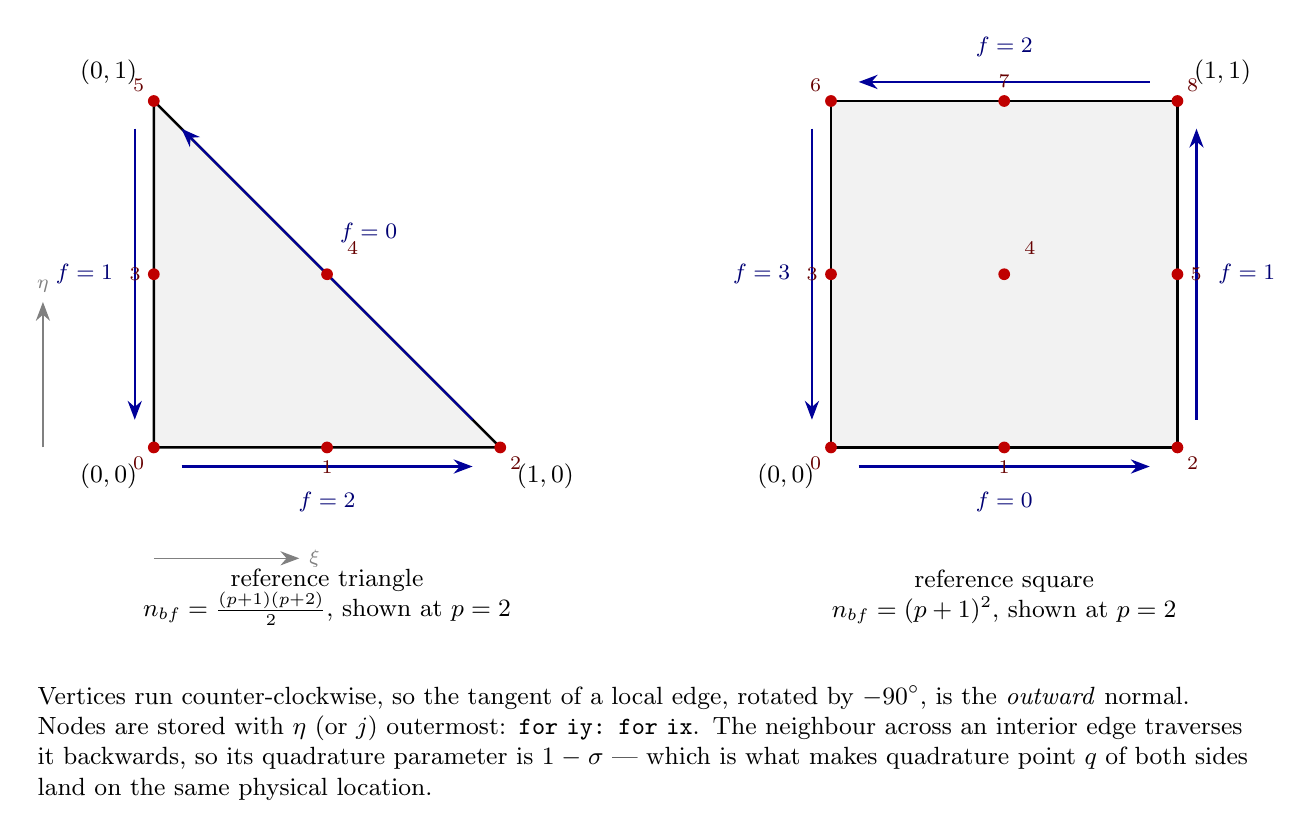
\begin{tikzpicture}[
  >={Stealth[length=2.4mm]},
  node distance=0pt,
  edgearr/.style = {->, blue!60!black, line width=0.8pt},
  nd/.style      = {circle, fill=red!75!black, inner sep=1.5pt},
  ndlbl/.style   = {font=\scriptsize, red!40!black},
  elbl/.style    = {font=\footnotesize, blue!45!black},
  vlbl/.style    = {font=\small},
  capt/.style    = {font=\small},
]

%% ------------------------------------------------------------------ TRIANGLE
\begin{scope}[scale=4.4]
  \fill[black!5] (0,0) -- (1,0) -- (0,1) -- cycle;
  \draw[line width=0.9pt] (0,0) -- (1,0) -- (0,1) -- cycle;

  % local edges: edge f is opposite vertex f, traversed CCW
  \draw[edgearr] (0.92,0.08) -- (0.08,0.92);      % f = 0 : v1 -> v2
  \draw[edgearr] (-0.055,0.92) -- (-0.055,0.08);  % f = 1 : v2 -> v0
  \draw[edgearr] (0.08,-0.055) -- (0.92,-0.055);  % f = 2 : v0 -> v1
  \node[elbl] at (0.62,0.62) {$f=0$};
  \node[elbl, anchor=east] at (-0.09,0.5) {$f=1$};
  \node[elbl, anchor=north] at (0.5,-0.10) {$f=2$};

  % p = 2 Lagrange nodes, in storage order
  \foreach \p/\i in {{0,0}/0, {0.5,0}/1, {1,0}/2, {0,0.5}/3, {0.5,0.5}/4, {0,1}/5}
    { \node[nd] at (\p) {}; }
  \node[ndlbl, anchor=north east] at (0,0)      {$0$};
  \node[ndlbl, anchor=north]      at (0.5,-0.01){$1$};
  \node[ndlbl, anchor=north west] at (1,0)      {$2$};
  \node[ndlbl, anchor=east]       at (-0.01,0.5){$3$};
  \node[ndlbl, anchor=south west] at (0.53,0.53){$4$};
  \node[ndlbl, anchor=south east] at (0,1)      {$5$};

  \node[vlbl, anchor=north east] at (-0.02,-0.02) {$(0,0)$};
  \node[vlbl, anchor=north west] at (1.02,-0.02)  {$(1,0)$};
  \node[vlbl, anchor=south east] at (-0.02,1.02)  {$(0,1)$};

  \draw[->, gray, line width=0.5pt] (0,-0.32) -- (0.42,-0.32)
        node[right, font=\scriptsize, gray] {$\xi$};
  \draw[->, gray, line width=0.5pt] (-0.32,0) -- (-0.32,0.42)
        node[above, font=\scriptsize, gray] {$\eta$};
\end{scope}

\node[capt, align=center] at (2.2,-1.9)
  {reference triangle\\ $n_{bf} = \tfrac{(p+1)(p+2)}{2}$, shown at $p=2$};

%% ------------------------------------------------------------------ QUAD
\begin{scope}[xshift=8.6cm, scale=4.4]
  \fill[black!5] (0,0) rectangle (1,1);
  \draw[line width=0.9pt] (0,0) rectangle (1,1);

  \draw[edgearr] (0.08,-0.055) -- (0.92,-0.055);   % f = 0
  \draw[edgearr] (1.055,0.08) -- (1.055,0.92);     % f = 1
  \draw[edgearr] (0.92,1.055) -- (0.08,1.055);     % f = 2
  \draw[edgearr] (-0.055,0.92) -- (-0.055,0.08);   % f = 3
  \node[elbl, anchor=north] at (0.5,-0.10) {$f=0$};
  \node[elbl, anchor=west]  at (1.09,0.5)  {$f=1$};
  \node[elbl, anchor=south] at (0.5,1.10)  {$f=2$};
  \node[elbl, anchor=east]  at (-0.09,0.5) {$f=3$};

  \foreach \x in {0,0.5,1}
    \foreach \y in {0,0.5,1}
      { \node[nd] at (\x,\y) {}; }
  \node[ndlbl, anchor=north east] at (0,0)       {$0$};
  \node[ndlbl, anchor=north]      at (0.5,-0.01) {$1$};
  \node[ndlbl, anchor=north west] at (1,0)       {$2$};
  \node[ndlbl, anchor=east]       at (-0.01,0.5) {$3$};
  \node[ndlbl, anchor=south west] at (0.53,0.53) {$4$};
  \node[ndlbl, anchor=west]       at (1.01,0.5)  {$5$};
  \node[ndlbl, anchor=south east] at (0,1)       {$6$};
  \node[ndlbl, anchor=south]      at (0.5,1.01)  {$7$};
  \node[ndlbl, anchor=south west] at (1,1)       {$8$};

  \node[vlbl, anchor=north east] at (-0.02,-0.02) {$(0,0)$};
  \node[vlbl, anchor=south west] at (1.02,1.02)   {$(1,1)$};
\end{scope}

\node[capt, align=center] at (10.8,-1.9)
  {reference square\\ $n_{bf} = (p+1)^2$, shown at $p=2$};

\node[capt, align=left, anchor=north west, text width=15.6cm] at (-1.6,-2.9)
  {Vertices run counter-clockwise, so the tangent of a local edge, rotated by
   $-90^\circ$, is the \emph{outward} normal.  Nodes are stored with
   $\eta$ (or $j$) outermost: \texttt{for iy: for ix}.  The neighbour across an
   interior edge traverses it backwards, so its quadrature parameter is
   $1-\sigma$ --- which is what makes quadrature point $q$ of both sides land on
   the same physical location.};

\end{tikzpicture}

\end{document}
